% Chapter 3
\let\cleardoublepage\clearpage
 % \let\cleardoublepage\clearpage
\chapter{Methdology} % Main chapter title

\label{Chapter3} % For referencing the chapter elsewhere, use \ref{Chapter1} 

%----------------------------------------------------------------------------------------

% Define some commands to keep the formatting separated from the content 
\newcommand{\keyword}[1]{\textbf{#1}}
\newcommand{\tabhead}[1]{\textbf{#1}}
\newcommand{\code}[1]{\texttt{#1}}
\newcommand{\file}[1]{\texttt{\bfseries#1}}
\newcommand{\option}[1]{\texttt{\itshape#1}}


\section{Data Collection}

In the pursuit of building an effective credit card fraud detection system, a critical initial step involves the collection and understanding of the data that will fuel the model's learning. This section outlines the process of importing necessary libraries, loading the dataset, and gaining insights into its structure.\medskip

In the context of machine learning, the effectiveness of our model is highly dependent on the quality of the dataset we use. Prior to delving into the nuances of model development, a pivotal phase involves the preprocessing of your dataset. This encompasses addressing missing values, handling duplicates, and transforming variables into a format that is conducive for model comprehension. This chapter delves into the intricate steps of data preprocessing undertaken for a credit card fraud detection project.

\subsection{Data Sources}

The project will utilize real credit card transaction data obtained from the kaggle which contains transactions made by credit cards in September 2013 by European cardholders.This dataset presents transactions that occurred in two days, where we have 492 frauds out of 284,807 transactions. The dataset is highly unbalanced, the positive class (frauds) account for 0.172\% of all transactions.\medskip

It contains only numerical input variables which are the result of a PCA transformation. Unfortunately, due to confidentiality issues, we cannot provide the original features and more background information about the data. Features V1, V2, … V28 are the principal components obtained with PCA, the only features which have not been transformed with PCA are 'Time' and 'Amount'. Feature 'Time' contains the seconds elapsed between each transaction and the first transaction in the dataset. The feature 'Amount' is the transaction Amount, this feature can be used for example-dependant cost-sensitive learning. Feature 'Class' is the response variable and it takes value 1 in case of fraud and 0 otherwise.

\subsection{Data Preprocessing}
\begin{itemize}
    \item \textbf{Data Cleaning:-} Before diving into the heart of the analysis, it's essential to ensure that the dataset is free from inconsistencies, missing values, and anomalies that could hinder the performance of our fraud detection system.

    \item \textbf{Feature Selection:-} Identifying the most relevant features (variables) is key to building an efficient model. This involves understanding the significance of each attribute and its potential contribution to the detection of fraudulent transactions.

    \item \textbf{Handling Imbalanced Data:-} Credit card fraud datasets often suffer from class imbalance, where the number of non-fraudulent transactions far exceeds fraudulent ones. Balancing the dataset is crucial to avoid the model being biased towards the majority class.

    \item \textbf{ Data Normalization:-}  Ensuring uniform scales across features is essential for certain machine learning algorithms. In the case of credit card fraud detection, normalizing the data aids in better convergence during the model training process.
    
\begin{figure}[h]
    \centering
    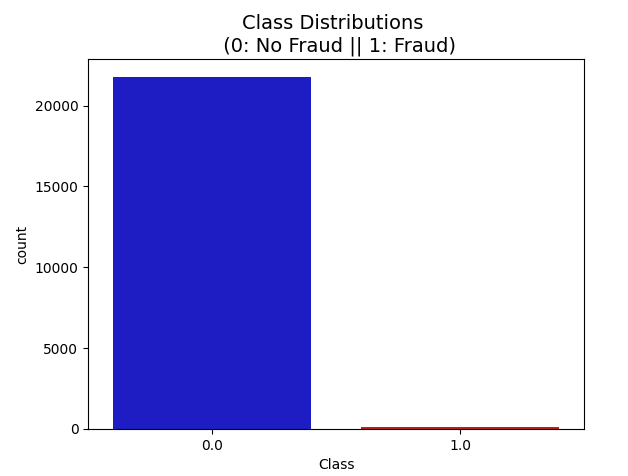
\includegraphics[width=0.7\linewidth]{image2.png}
    \caption{Class Distribution}
    \label{fig:enter-label}
\end{figure}

\item \textbf{ Scaling and Distributing :-}In this phase of our kernel, we will first scale the columns comprise of Time and Amount . Time and amount should be scaled as the other columns. On the other hand, we need to also create a sub sample of the dataframe in order to have an equal amount of Fraud and Non-Fraud cases, helping our algorithms better understand patterns that determines whether a transaction is a fraud or not.

 \begin{figure}[h]
    \centering
    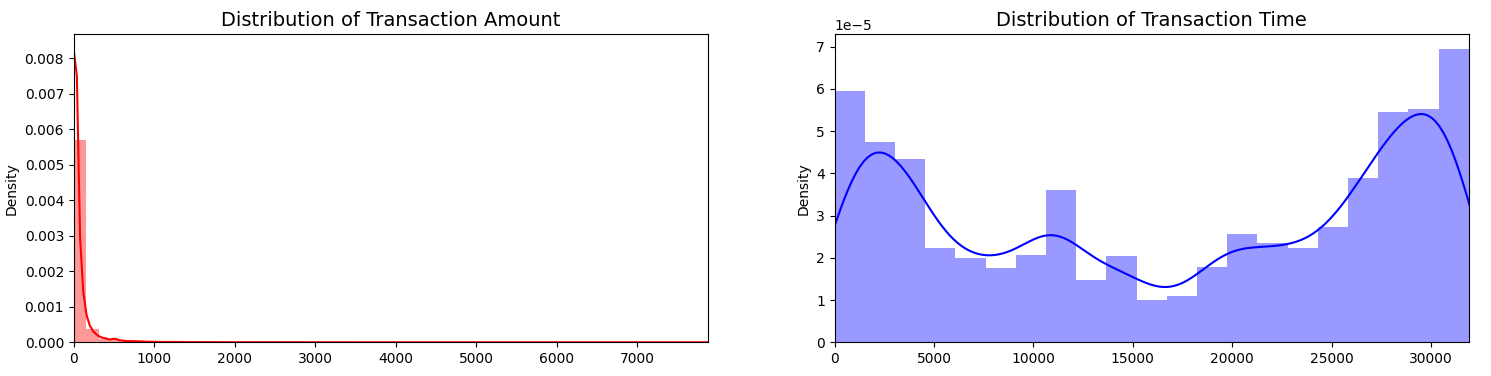
\includegraphics[width=0.8\linewidth]{image3.png}
    \caption{Distribution}
    \label{fig:enter-label}
 \end{figure}

\item \textbf{ Splitting Data:-}Before proceeding with the Random UnderSampling technique we have to separate the orginal dataframe. Why? for testing purposes, remember although we are splitting the data when implementing Random UnderSampling or OverSampling techniques, we want to test our models on the original testing set not on the testing set created by either of these techniques. The main goal is to fit the model either with the dataframes that were undersample and oversample (in order for our models to detect the patterns), and test it on the original testing set.

\end{itemize}

\section{Feature Selection/Engineering}

The process of identifying the most influential features and potentially creating new ones is critical for developing a robust credit card fraud detection model. This section delves into the methods employed for feature selection and engineering to enhance the overall efficacy of the model.\medskip

In my code, explicit feature selection techniques are not applied. Instead, the focus is on outlier detection and removal, correlation analysis, and subsampling to address class imbalance. Let's discuss how feature-related aspects are handled in the code.

\begin{itemize}
    \item \textbf{Feature Importance:-} Determining the importance of each feature provides insights into which variables significantly contribute to the identification of fraudulent transactions. Random Forest Classifier, being an ensemble method, inherently provides a mechanism to gauge feature importance.
    
    \item Correlation matrices (corr and sub\_sample\_corr) are used to visualize the correlation between features and the target variable ('Class').
    \item Features with high positive or negative correlations with the target variable are identified.
    \begin{figure}[h]
        \centering
        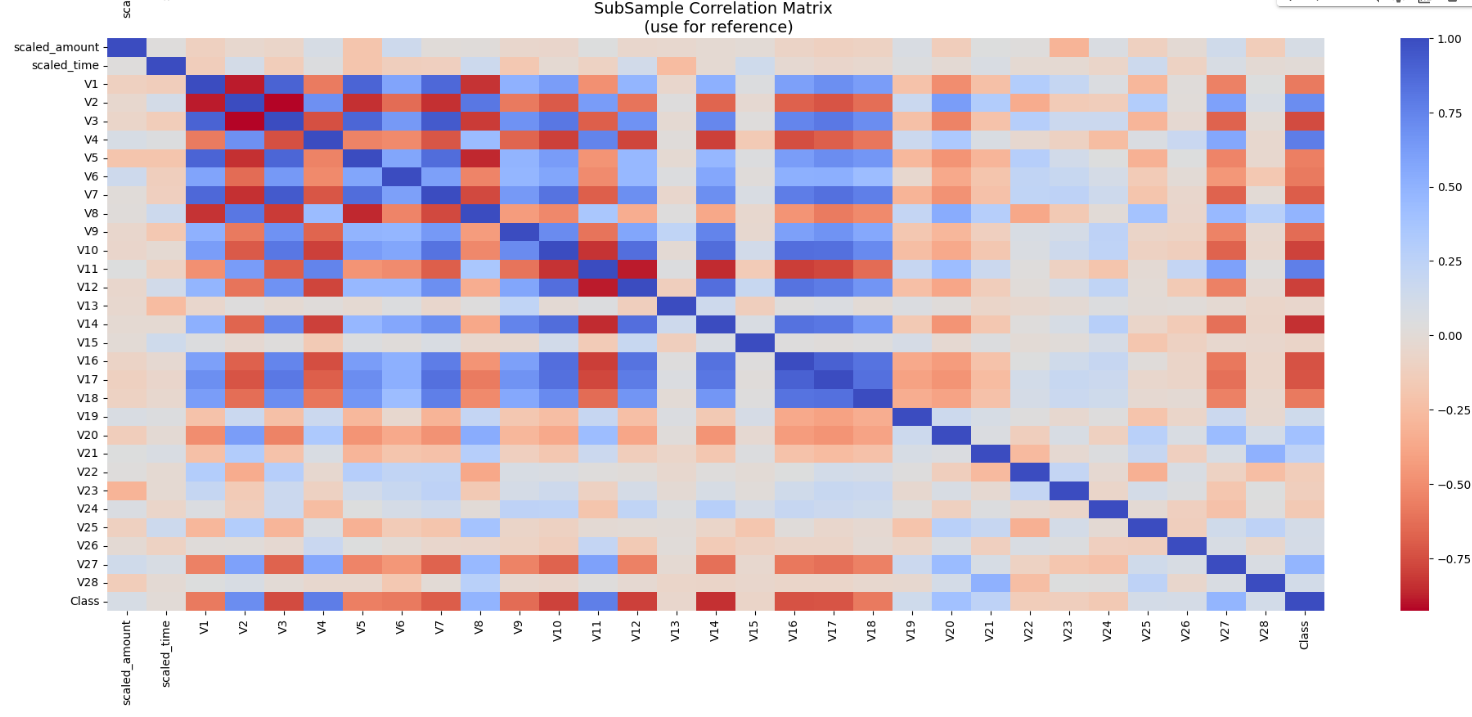
\includegraphics[width=0.9\linewidth]{image4.png}
        \caption{SubSample Correlation Matrix}
        \label{fig:enter-label}
    \end{figure}
    \item Boxplots are created to show the distribution of features with the highest negative and positive correlations.

  \item \textbf{Feature Engineering:-} Creating new features based on existing ones can uncover hidden patterns and improve the model's ability to discern fraudulent transactions.

  Feature selection and engineering are iterative processes, and the chosen techniques depend on the dataset and the behavior of fraudulent transactions. The selected features and engineered variables form the foundation for training and optimizing the Random Forest Classifier and Logistic Regression in the subsequent stages of the project.
   \begin{figure}[h]
       \centering
       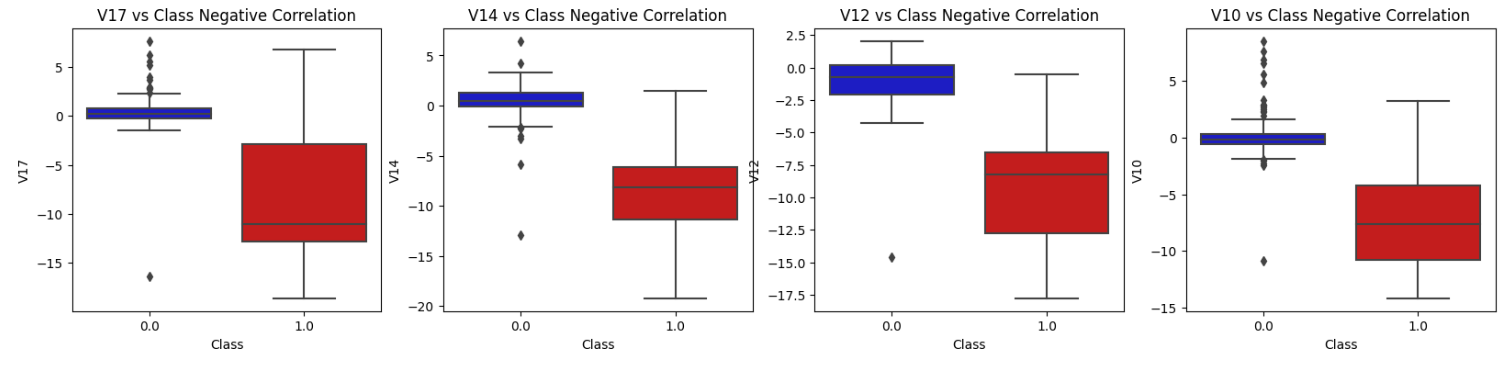
\includegraphics[width=0.9\linewidth]{image5.png}
       \caption{Negative Correlation With Classes}
       \label{fig:enter-label}
   \end{figure}
   \item \textbf{Outlier Detection:} Outlier detection in credit card fraud detection involves identifying and handling transactions that deviate significantly from the typical behavior of legitimate transactions. Outliers in this context are often indicative of potential fraudulent activity. 
   \item Outlier removal is performed for features V14, V12, and V10 using the interquartile range (IQR) method.
   
   \begin{figure}[h]
    \centering
    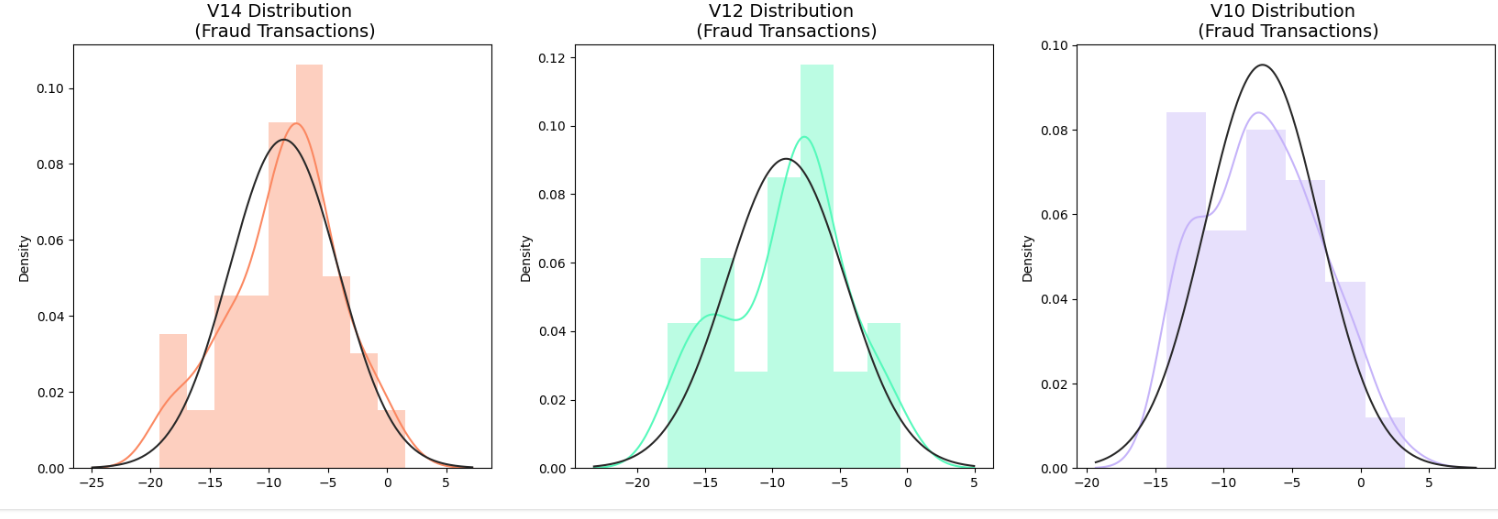
\includegraphics[width=0.9\linewidth]{image6.png}
    \caption{Fraud Transaction}
    \label{fig:enter-label}
\end{figure}

   \item The reduction in extreme outliers is visualized using boxplots.
   
   \begin{figure}[h]
       \centering
       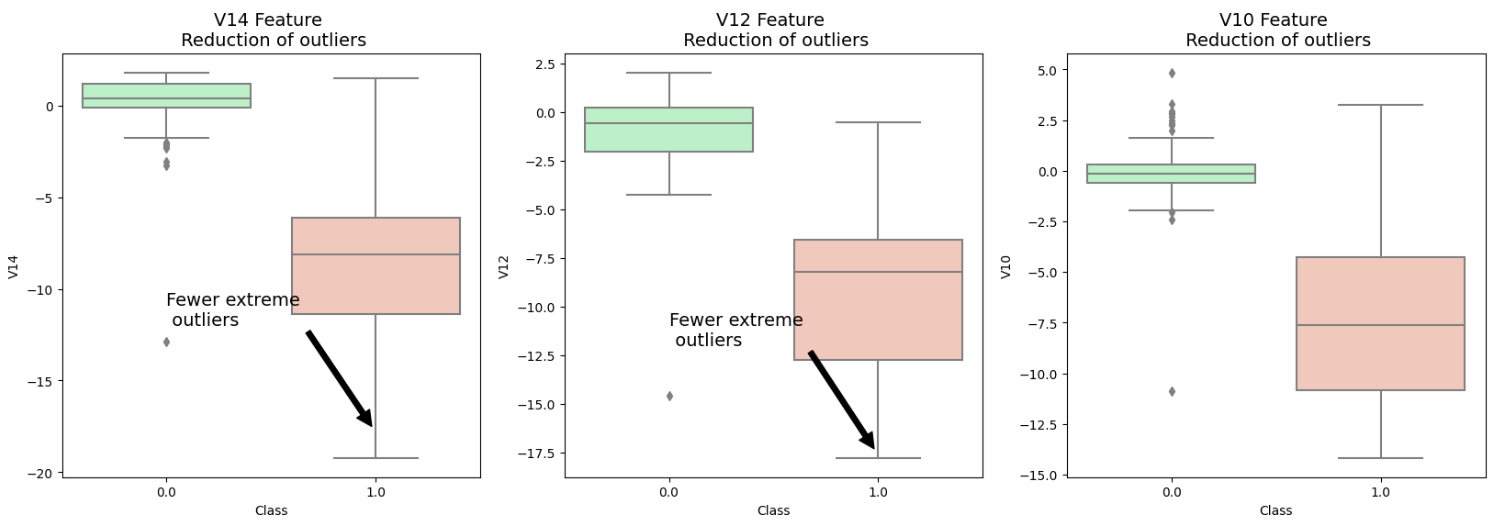
\includegraphics[width=0.9\linewidth]{image7.png}
       \caption{Reduction of Outliers}
       \label{fig:enter-label}
   \end{figure}

   \item \textbf{Subsampling:} Subsampling in the context of credit card fraud detection involves creating a balanced dataset by randomly selecting a subset of legitimate transactions to match the number of fraudulent transactions. This technique is often employed when dealing with imbalanced datasets, where fraudulent transactions are significantly less frequent than legitimate ones. 
   \item Random under-sampling is applied to balance the class distribution, ensuring an equal number of fraud and non-fraud instances.
   \item This subsample is then used for further analysis and model training.\medskip
   
  \item \textbf{Dimensionality Reduction and Clustering:} 
The dimensionality reduction techniques of t-SNE, PCA, and Truncated SVD were employed to visualize clusters in the credit card fraud dataset. The scatter plots showcase distinct clusters that differentiate between legitimate transactions (labeled as 'No Fraud') and fraudulent transactions (labeled as 'Fraud'). In the t-SNE plot, clusters exhibit a well-defined separation, highlighting the ability of t-SNE to capture complex patterns in high-dimensional data. PCA also effectively distinguishes between the two classes, revealing clusters with clear boundaries. Truncated SVD, while offering dimensionality reduction, demonstrates slightly overlapping clusters, indicating some level of complexity in the underlying data structure. The use of different dimensionality reduction techniques provides valuable insights into the distribution of fraud and non-fraud instances, aiding in the identification of patterns crucial for fraud detection in the credit card transactions dataset.

\begin{figure}[h]
    \centering
    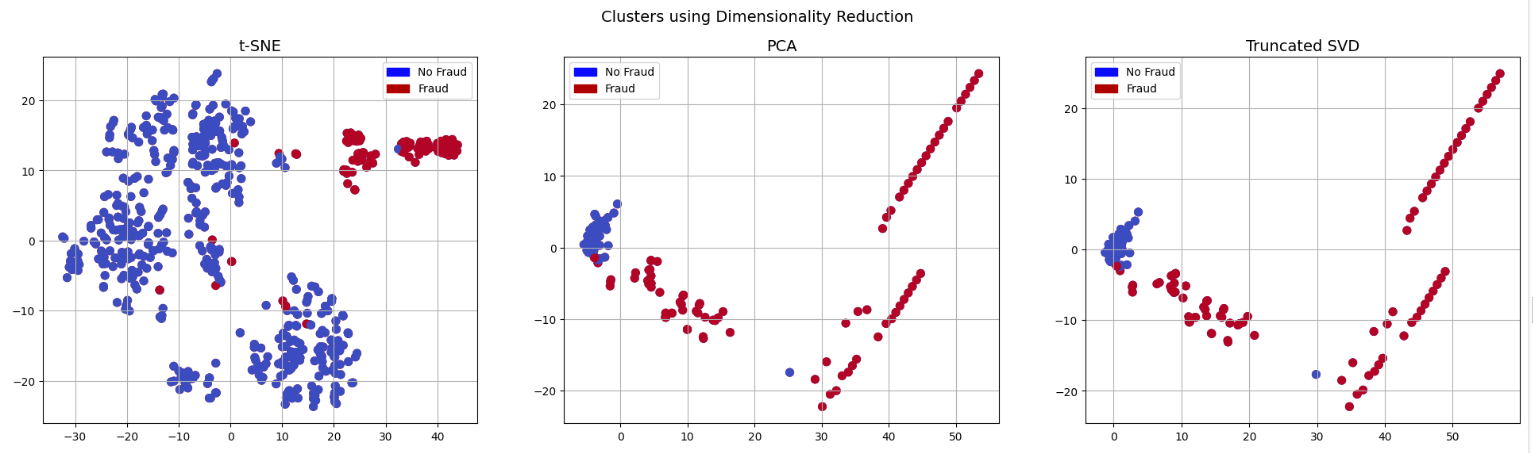
\includegraphics[width=0.9\linewidth]{image8.png}
    \caption{Clusters using Diamensionality}
    \label{fig:enter-label}
\end{figure}

   

\end{itemize}

\section{Model Selection:-} In credit card fraud detection, the choice of an appropriate model plays a pivotal role in achieving accurate and efficient results. The Random Forest Classifier and Logistic Regression stands out as a formidable choice due to its ability to handle complex patterns, manage large datasets, and mitigate overfitting, all crucial aspects in the context of identifying fraudulent transactions. Comprising an ensemble of decision trees, the Random Forest algorithm excels in capturing intricate relationships within the data, making it well-suited for the dynamic and evolving nature of credit card fraud. Leveraging the strength of multiple trees, it excels in delivering robust predictions and is inherently resistant to outliers and noise. The adaptability and resilience of the Random Forest Classifier position it as a reliable tool for our credit card fraud detection endeavor, promising to provide a nuanced understanding of transaction patterns and effectively differentiate between legitimate and fraudulent activities.\medskip

Logistic regression stands as a powerful ally in the ongoing battle against credit card fraud. Its simplicity, interpretability, and efficiency make it a valuable tool for financial institutions striving to protect their customers and maintain the integrity of electronic transactions. As technology evolves, logistic regression remains a steadfast and reliable solution in the realm of fraud detection.

\section{Evaluation:-} After the training phase, assessing the performance of the credit card fraud detection model is crucial to ensuring its efficacy in real-world scenarios. This section discusses the evaluation process and the metrics employed to gauge the model's success in accurately identifying fraudulent transactions.

\begin{itemize}

    \item \textbf{Accuracy:-} Accuracy represents the proportion of correctly classified instances, measuring the overall correctness of the model's predictions.This suggests that, during cross-validation on the training data, the Logistic Regression model achieved an accuracy of 85.0\% where the Random Forest give accuracy is 79\%. This high accuracy score indicates that, based on the training data, the Logistic Regression model is performing well in predicting whether transactions are fraudulent or not.

 \begin{figure}[h]
     \centering
     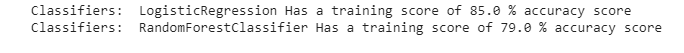
\includegraphics[width=0.9\linewidth]{image9.png}
     \caption{Accuracy Score}
     \label{fig:enter-label}
 \end{figure}
 
    \item \textbf{Precision and Recall:-} Precision and recall are particularly relevant in fraud detection. Precision measures the accuracy of positive predictions, while recall gauges the model's ability to capture all positive instances.\medskip
    
    \begin{figure}[h]
        \centering
        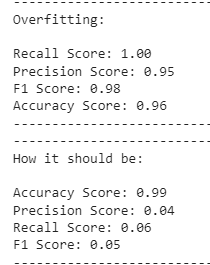
\includegraphics[width=0.5\linewidth]{image11.png}
        \caption{Precision and Recall score of LR}
        \label{fig:enter-label}
    \end{figure}
    
    This suggests that the ROC AUC score for the Logistic Regression model on the training data is 0.96 where the Random Forest gave 0.95, indicating a strong ability of the model to distinguish between positive and negative classes (fraudulent and legitimate transactions). Higher ROC AUC values generally imply better model performance.
    
    \begin{figure}[h]
        \centering
        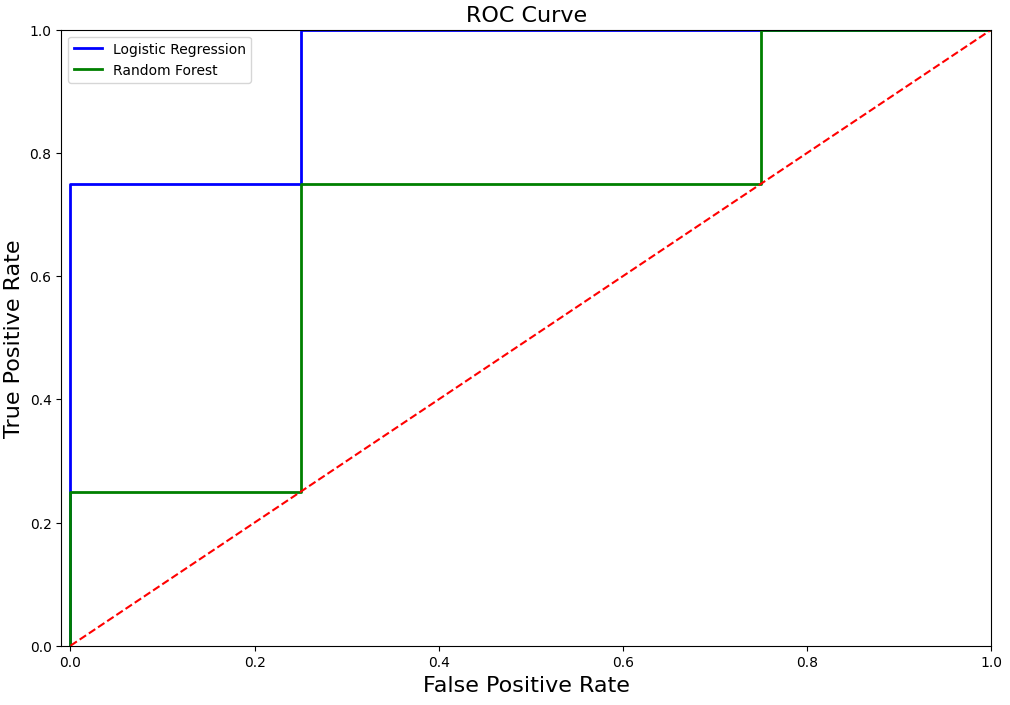
\includegraphics[width=0.9\linewidth]{image10.png}
        \caption{ROC Curve of LR and RF}
        \label{fig:enter-label}
    \end{figure}

    \item \textbf{Confusion Matrix:-} A confusion matrix provides a detailed breakdown of true positive, true negative, false positive, and false negative instances.These metrics collectively provide a comprehensive assessment of the model's performance in credit card fraud detection.\medskip
     Logistic Regression classifier, illustrating the true positive, true negative, false positive, and false negative predictions on the training data. The heatmap provides a visual representation of the performance of the Logistic Regression model in classifying fraudulent and legitimate transactions.
     
     \begin{figure}[h]
         \centering
         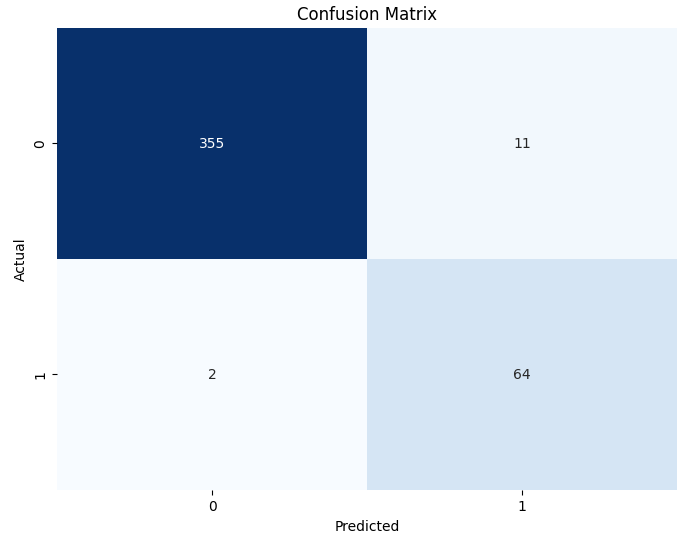
\includegraphics[width=0.7\linewidth]{image12.png}
         \caption{Confusion Matrix of LR}
         \label{fig:enter-label}
     \end{figure}

    \item \textbf{Validation:-} Validation ensures that the trained model generalizes well to new, unseen data. In our case, we employ cross-validation to assess the model's robustness.

    \item \textbf{Implementation:-} With a tuned and validated Random Forest Classifier, the next step is the real-world implementation of the model into the credit card company's existing systems.

    Validation, and Implementation stages collectively elevate the Random Forest Classifier to its maximum potential in safeguarding against credit card fraud.

    \item \textbf{Monitoring and Maintenance:-} The implementation of the credit card fraud detection system doesn't end with deployment. Continuous monitoring and proactive maintenance are vital to ensure the model's sustained effectiveness in the ever-evolving landscape of fraudulent activities.

\end{itemize}


